\section{Estudo Exprimental}

Para alcançar o objetivo de identificar quantos warnings das ferramentas CogniCrypt e CryptoGuard advém ou não de uma biblioteca extena, adotamos a abordagem GQM (Goal, Question, Metric), conforme descrito a seguir:

\subsection{Estrutura da Metodologia (GQM)}

\subsection{Objetivo}

Identificar a quantidade de \textit{warnings} das ferramentas CogniCrypt e CryptoGuard que advém de bibliotecas externas. 

\subsubsection{Questões de Pesquisa}
Definimos as seguintes perguntas baseadas nos dados coletados:

\begin{itemize}
\item \textbf{RQ1:} Qual é a quantidade de \textit{warnings} no \textit{dataset} de aplicativos Android analisados pelas ferramentas CogniCrypt e CryptoGuard?

\item \textbf{RQ2:} Qual o percentual de \textit{warnings} específicos de bibliotecas externas?

\item \textbf{RQ3:} Dado as limitações de análise da ferramenta LibScout, qual o percentual de \textit{warnings} que possivelmente são de bibliotecas externas?

\end{itemize}

\subsubsection{Métricas}
Para responder as questões RQ1, RQ2 e RQ3 as seguintes métricas foram estabelecidas:

\begin{itemize}
\item \textbf{M1: Número total de warnings detectados pela ferramenta CogniCrypt.} \
Nos 307 aplicativos analisados, após executar o CogniCrypt, a ferramenta identificou 11.036 \textit{warnings} de crypto api missuses.

\item \textbf{M2: Número total de warnings detectados pela ferramenta CriptoGuard.} \
Nos mesmos aplicativos analisados pelo CogniCrypt, a ferramenta CryptoGuard identificou 4.964 \textit{warnings}. Essas métricas são essenciais para quantificar a presença geral de vulnerabilidades no conjunto de dados de aplicativos Android.


\item \textbf{M3: Número total de bibliotecas externas na ferramenta CogniCrypt.} \

No CogniCrypt, de um total de 6.798 bibliotecas contabilizadas dos 307 aplicativos, a ferramenta LibScout identificou que 1.710 \textit{warnings} advém de bibliotecas externas.

\item \textbf{M4: Número total de bibliotecas externas na ferramenta CriptoGuard.} \

No CryptoGuard, de um total de 2.710 bibliotecas dos mesmos 307 aplicativos, o LibScout identificou que 1.149 \textit{warnings} advém de bibliotecas externas. 

Isso demonstra que uma parte considerável dos \textit{warnings} detectados pode ser atribuída a bibliotecas externas, o que sugere a importancia da integração dessas ferramentas na identificação da origem dos \textit{warnings} e na detecção de vulnerabilidades específicas de bibliotecas externas.

Com o resultado da integração do resultado do LibScout com os \textit{warnings} identificados pelo CogniCrypt e CriptoGuard criamos uma abordagem capaz de identificar os \textit{warnings} associados a bibliotecas externas daqueles associados a bibliotecas nativas.

\item \textbf{M5: Número total de bibliotecas possivelmente externas na ferramenta CogniCrypt} \

Após a integração dos resultados do LibScout com os \textit{warnings} identificados por ambas as ferramentas, observamos que apesar do LibScout gerar resultados com precisão de algumas bibliotecas externas, a ferramenta não é capaz de identificar todas as bibliotecas externas presentes nos aplicativos \cite{api_tpl_zhang}.

Para melhorar a precisão dos resultados, identificamos também as bibliotecas que estão presentes nos aplicativos, mas que não foram detectadas pelo LibScout como bibliotecas externas. Uma biblioteca reconhecida pelo LibScout e presente nos resultados das ferramentas de análise estática foram marcadas como possivelmente externas e foram incluídas na análise.

Das 6.798 bibliotecas identificadas pelo CogniCrypt, 726 foram marcadas como possivelmente externas.

\item \textbf{M6: Número total de bibliotecas possivelmente externas na ferramenta CriptoGuard} \

Já das 2.710 bibliotecas identificadas pelo CryptoGuard, 245 foram marcadas como possivelmente externas.


\end{itemize}

\subsection{Metodologia do Estudo}

Para conseguir essas métricas e responder às questões de pesquisa, a pesquisa foi dividida em várias fases, conforme descrito a seguir:

\begin{itemize}
\item \textbf{Coleta de Dados:} Inicialmente, foi coletado um conjunto de aplicativos Android de código aberto para análise. O conjunto de dados foi obtido do repositório F-Droid, que contém aplicativos de código aberto disponíveis para download. O repositório foi escolhido devido à sua natureza de código aberto e à disponibilidade de aplicativos para download. Então foi executado o CogniCrypt e o CryptoGuard em cada aplicativo para identificar vulnerabilidades em APIs criptográficas.

\item \textbf{Análise de vulnerabilidades e alerta aos desenvolvedores:} Em seguida, foram utilizadas as ferramentas CogniCrypt e CryptoGuard para analisar os aplicativos e identificar vulnerabilidades em APIs criptográficas. As ferramentas foram escolhidas devido à sua capacidade de detectar vulnerabilidades em APIs criptográficas e fornecer alertas aos desenvolvedores sobre possíveis problemas de segurança. Nessa etapa, identificamos que vários dos \textit{warnings} detectados pelas ferramentas estavam associados a código que os desenvolvedores não tinham escrito e sim a códigos de bibliotecas externas. 

\item \textbf{Identificação e Seleção das Ferramentas:} Para identificar as bibliotecas externas, fizemos uma análise da literatura e através do estudo realizado por \cite{api_tpl_zhang}, identificamos o LibScout como uma ferramenta eficaz para identificar bibliotecas em aplicativos Android. O LibScout foi escolhido devido à sua capacidade de identificar bibliotecas em aplicativos Android e fornecer informações detalhadas sobre as bibliotecas encontradas. O estudo cita outras ferramentas que poderiam ser utilizadas, como o LibRadar, LibID, libPecker, entre outros. O LibRadar foi um dos aplicativos inicialmente considerados para podermos comparar com os resutlados do LibScout, no entanto, o número de bibliotecas externas encotradas em um subset dos quais já sabiamos os resultados não foi suficiente. O LibRadar compara os resultados da investigação com um dataset base, o qual não foi atualizado nos últimos 7 anos. Cada uma das ferramentas destacadas no paper de Zhang tem suas limitações, como a falta de atualizações de datasets, tempo exagerado para análise de apenas um aplicativo, baixa confiabilidade nos resultados. De todas as métricas descritas no artigo, o LibScout foi a que apresentava resultados mais confiáveis em tempo hábil para análise de um grande número de aplicativos. 

\item \textbf{Integração das Ferramentas:} Após a seleção, integramos os resultados do LibScout aos contextos das ferramentas CryptoGuard e CogniCrypt. Essa integração permitiu uma análise mais detalhada e contextualizada das vulnerabilidades encontradas, especialmente em bibliotecas externas.

\item \textbf{Execução do Experimento:} O experimento foi realizado em várias etapas, incluindo a caracterização do dataset, a coleta de dados, e a análise dos resultados. Durante a análise, geramos gráficos e tabelas para ilustrar a distribuição de \textit{warnings} e a prevalência de vulnerabilidades, conforme descrito no próximo capítulo.

\end{itemize}

\begin{figure}[!ht]
  \centering
  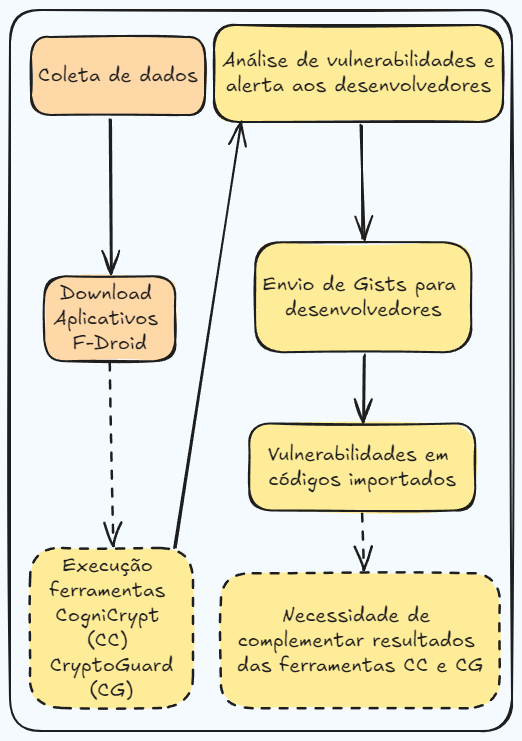
\includegraphics[scale=0.4]{img/research_steps1.png}
  \caption{Fases da pesquisa}
  \label{img: research_steps}
\end{figure}

\begin{figure}[!ht]
  \centering
  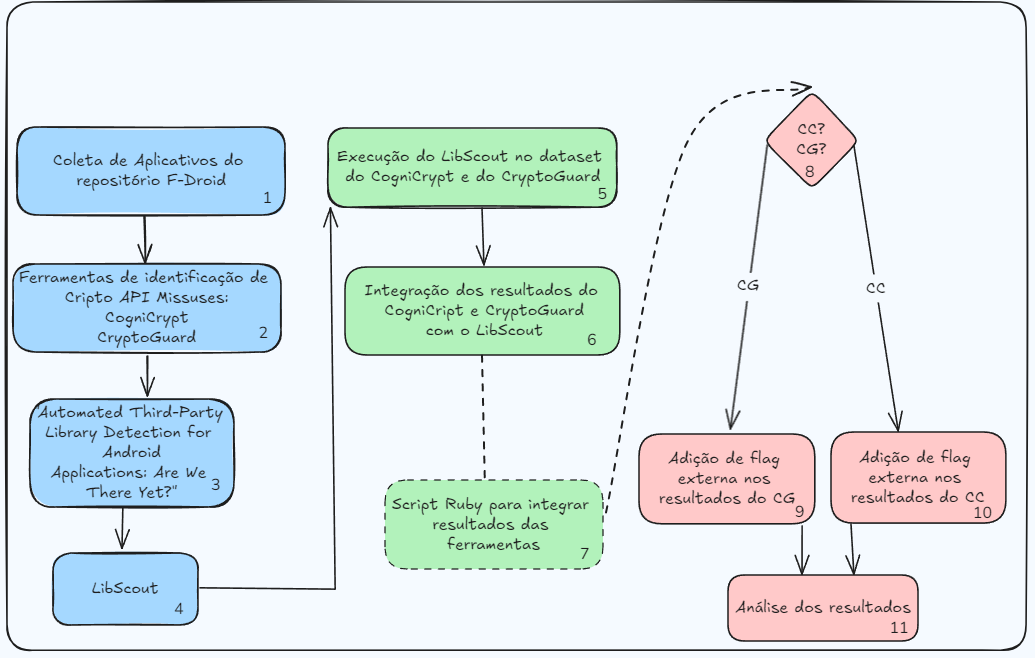
\includegraphics[scale=0.4]{img/research_steps2.png}
  \caption{Fases da pesquisa}
  \label{img: research_steps2}
\end{figure}